%\documentclass[times]{itmo-student-thesis}
\documentclass[specification,annotation]{itmo-student-thesis}

%% Опции пакета:
%% - specification - если есть, генерируется задание, иначе не генерируется
%% - annotation - если есть, генерируется аннотация, иначе не генерируется
%% - times - делает все шрифтом Times New Roman, собирается с помощью xelatex
%% - pscyr - делает все шрифтом Times New Roman, требует пакета pscyr.

%% Делает запятую в формулах более интеллектуальной, например:
%% $1,5x$ будет читаться как полтора икса, а не один запятая пять иксов.
%% Однако если написать $1, 5x$, то все будет как прежде.
%\usepackage{icomma}

%% Один из пакетов, позволяющий делать таблицы на всю ширину текста.
\usepackage{tabularx}

%% Данные пакеты необязательны к использованию в бакалаврских/магистерских
%% Они нужны для иллюстративных целей
%% Начало
\usepackage{tikz}
\usetikzlibrary{arrows}
\usepackage{filecontents}
\usepackage{mathtools}
\DeclarePairedDelimiter{\ceil}{\lceil}{\rceil}

\begin{filecontents}{master-thesis.bib}
@incollection{ nsga-ii-steady-state,
    year        = {2009},
    booktitle   = {Nature-Inspired Algorithms for Optimisation},
    number      = {193},
    series      = {Studies in Computational Intelligence},
    title       = {On the Effect of Applying a Steady-State Selection Scheme in the Multi-Objective Genetic Algorithm {NSGA}-{II}},
    publisher   = {Springer Berlin Heidelberg},
    author      = {Nebro, Antonio J. and Durillo, Juan J.},
    pages       = {435-456},
    langid      = {english}
}


@inproceedings{ example-english,
    year        = {2015},
    booktitle   = {Proceedings of IEEE Congress on Evolutionary Computation},
    author      = {Maxim Buzdalov and Anatoly Shalyto},
    title       = {Hard Test Generation for Augmenting Path Maximum Flow 
                   Algorithms using Genetic Algorithms: Revisited},
    pages       = {2121-2128},
    langid      = {english}
}

@article{ example-russian,
    author      = {Максим Викторович Буздалов},
    title       = {Генерация тестов для олимпиадных задач по программированию 
                   с использованием генетических алгоритмов},
    journal     = {Научно-технический вестник {СПбГУ} {ИТМО}},
    number      = {2(72)},
    year        = {2011},
    pages       = {72-77},
    langid      = {russian}
}

@article{ unrestricted-jump-evco,
    author      = {Maxim Buzdalov and Benjamin Doerr and Mikhail Kever},
    title       = {The Unrestricted Black-Box Complexity of Jump Functions},
    journal     = {Evolutionary Computation},
    year        = {2016},
    note        = {Accepted for publication},
    langid      = {english}
}

@book{ bellman,
    author      = {R. E. Bellman},
    title       = {Dynamic Programming},
    address     = {Princeton, NJ},
    publisher   = {Princeton University Press},
    numpages    = {342},
    pagetotal   = {342},
    year        = {1957},
    langid      = {english}
}
\end{filecontents}

%% Указываем файл с библиографией.
\addbibresource{master-thesis.bib}

\begin{document}

\studygroup{M4238}
\title{Разработка алгоритма консенсуса на основе комитета участников}
\author{Пересадин Илья Валерьевич}{Пересадин И.В.}
\supervisor{Шалыто Анатолий Абрамович}{Шалыто А.А.}{проф., д.т.н.}{главный научный сотрудник Университета ИТМО}
\publishyear{2019}
%% Дата выдачи задания. Можно не указывать, тогда надо будет заполнить от руки.
\startdate{01}{сентября}{2018}
%% Срок сдачи студентом работы. Можно не указывать, тогда надо будет заполнить от руки.
\finishdate{31}{мая}{2019}
%% Дата защиты. Можно не указывать, тогда надо будет заполнить от руки.
\defencedate{15}{июня}{2019}

\secretary{Павлова О.Н.}

%% Задание
%%% Техническое задание и исходные данные к работе
\technicalspec{В рамках данной работы требуется разработать и доказать алгоритм на основе комитета участников, который способен работать в инклюзивной модели.
Алгоритм должен решать проблемы присущие существующим аналогичным алгоритмам, быть эффективным и предоставлять высокии гарантии безопасности.
Требуется изучить последние достижения в этой области, проанализировать их проблемы и возможные пути решения. 
 }

%%% Содержание выпускной квалификационной работы (перечень подлежащих разработке вопросов)
\plannedcontents{
\begin{enumerate}
    \item Постановка задачи и обзор предметной области
    \item Описание предложенного алгоритма
    \item Анализ предложенного алгоритма
\end{enumerate}
}

%%% Исходные материалы и пособия 
\plannedsources{
\begin{enumerate}
    \item Miguel Castro, Practical Byzantine Fault Tolerance;
    \item Leslie Lamport, The Byzantine Generals Problem.
\end{enumerate}
}

%%% Цель исследования
\researchaim{Разработать эффективный и безопасный инклюзивный алгоритм консенсуса на основе комитета участников.} 

%%% Задачи, решаемые в ВКР
\researchtargets{
  \begin{enumerate}
    \item анализ алгоритмов консенсуса в существующих криптовалютах, их проблем и недостатков;
    \item описание алгоритма не имеющих данных проблем;
    \item доказательство описанного алгоритма;
    \item анализ устойчивости предложенного алгоритма к атакам.
  \end{enumerate}
}

%%% Использование современных пакетов компьютерных программ и технологий
\addadvancedsoftware{Использовалась система контроля версий Git и система компьютерной верстки LaTeX.}{\ref{chapter1}, \ref{chapter2}, \ref{chapter3}}

%%% Краткая характеристика полученных результатов 
\researchsummary{Разработан, доказан и проанализирован инклюзивный алгоритм консенсуса на основе комитета участников, который превосходит существующие по некоторым показателям. }

\researchfunding{
    Грантов или других форм государственной поддержи и субсидирования в процессе работы не предусматривалось.
}
 
\researchpublications{Работа была опубликована в журнале и в сборнике конференции
\begin{refsection}
\nocite{article-peresadin, conference-peresadin}
\printannobibliography
\end{refsection}
}

%% Эта команда генерирует титульный лист и аннотацию.
\maketitle{Магистр}

%% Оглавление
\tableofcontents

% Chapters
\startprefacepage
В последние годы криптовалюты набирали популярность как среди рядовых пользователей как альтернатива фиатным способам совершения платежей, а также как плодородная почва для исследования.
Большинство криптовалют реализованы таким образом, чтобы предоставить конечному пользователю ряд свойств и гарантий, которыми не обладают существующие фиатные финансовые институты. К таким свойствам относятся децентрализация, анонимность, безопаность и масштабируемость.
 
Достижение этих свойств одновремено зачастую является непростой задачей, 
поэтому они достигаются не в полной степени или с некотороми компромиссами.
Например, для достижения безопасности используются алгоритмы на основе доказательства работы (Proof of Work)\cite{pow}
что зачастую вызывает другие недостатки, такие как уменьшение скорости обработки транзакций или уязвимость к некоторым типам атак.
Другие же криптовалюты используют для обеспечения безопасности алгоритмы на основе доказательства доли владения (Proof of Stake)\cite{pos}, в которых 
возникают другие проблемы, такие как проблема "ничего на кону" (nothing-at-stake)\cite{pos},
что приводит к централизации криптовалюты.

%Актуальность
Одной из таких проблем современных криптовалют является скорость обработки транзакций. 
Например, Bitcoin способен обрабатывать лишь 7 транзакций в секунду. Данный недостаток вытекает из того,
что многие криптовалюты предоставляют только \textit{консистентность в конечном счете}\cite{DBLP:journals/corr/DeckerSW14}, то есть транзакции попавшие в блокчейн могут быть отменены, но утверждается, что в конечно счете, они окажутся в блокчейне. Данная гарантия была достаточной на рассвете зарождения технологии,  но является неудовлетворительной для текущих требований.

%Новизна
В данной работе будет предложен алгоритм консенсуса, который предоставляет строгии гарантии безопасности, 
вместе с тем высокую скорость обработки транзакций, в то же время оставаясь децентрализованным.
Преимуществом данного алгоритма также является то, что в нем не может быть откактов блоков,
что дает дополнительную гарантию, что однажды попавшая в блокчейн транзакция не может быть отменена.
Также в работе будет рассмотрено применение данного алгоритма как в сочетании с системой на основе доказательства выполненной работы,
так и с системой на основе доказательства долей владения.

% Структура работы
В главе 1 будут введены вспомогательные понятия, сформулированы решаемые задачи.
Также будет проведен обзор предметной области, существующие решения их недостатки и проблемы.

В главе 2 будут рассмотрены предложенные улучшения и их вариации, принцип работы и обоснование.

В главе 3 будет проведен анализ алгоритма, рассмотрены возможные атаки и показано, как алгоритм будет справляться с ними.
Также будут предоставлены результаты замеров скорости работы и потребляемой памяти.

%-*-coding: utf-8-*-

\graphicspath{ {images/} }

\startrelatedwork

\chapter{Обзор предметной области} \label{chapter1}
В данной главе проводится обзор предметной области.
Дается объяснение технологии <<блокчейн>>, понятия алгоритма консенсуса, транзакциях и
криптографических примитивов.
Далее следует рассмотрение существующих решений и описание их недостатков.

\section{Технология блокчейн}

Технология блокчейн, от английского blockchain, дословно переводится  как "цепочка блоков".

Блок хранит в себе данные, а также ссылку на предыдущий блок. 
Блоки образуют бесконечную последовательность, которая имеет начало, но не имеет конца.
Первый блок в блокчейне называется \textit{генезис блоком} (genesis block).

По сути блокченй представляет односвязный список, где каждый элемент знает ссылку на предыдущий. 
Однако, особенностью данного списка является то,  что в качестве ссылки на предыдущий блок 
используется хэш криптографически стойкой хэш-функции содержимого предыдущего блока, 
которое включает как его данные, так и ссылку на предыдущий блок. 
Поэтому даже при малейшей попытке заменить содержимое блока, 
поменяется значение хэш-функции его данных и ссылка на него от последующего блока будет недействительна.
Нахождение двух блоков с разным содержанием и одинаковым значением хэш-функции является  задачей, требующей экспоненциального количества вычислений. 
Таким образом, хэш последнего блока в цепочке является доказательством данной цепочки, то есть легко проверить что данный хэш соответствует цепочке, но создать другую цепочку с таким же хэшом является вычислительно сложной задачей. Данная особенность ключевая, и  является одной из основых для обеспечения безопасности в криптовалютах использующих технологию блокчейн.

\begin{figure}[h]
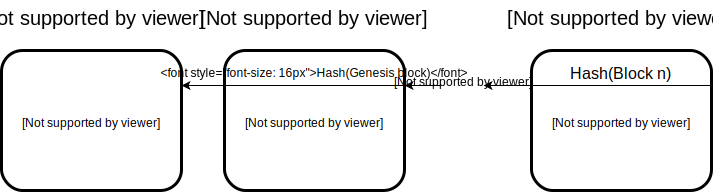
\includegraphics[scale=0.6]{Blockchain_Scheme}
\caption{\textbf{Схема блокчейна}}
\label{fig:blockchain}
\end{figure}

На Рисунке \ref{fig:blockchain} обозначено схематиченое представление блокчейна.

Будем называть описанную структуру ~--- блокчейн.

\section{Алгоритм достижения консенсуса}
Исследование в области распределенных систем началось задолго до  появление криптовалют, и насчитывает 30 лет исследования и разработки.
Алгоритмы достижения консенсуса между несколькими участниками ~--- являются одной из популярных задач в этой области.
Формально, класс таких алгоритмов можно описать следующим образом:
\par \textit{
Имеется $n$ участников, между которыми установлены каналы связи. Каждый участник знает некоторое число $x$ (у каждого свое).
После некоторой коммуникации по каналам связи они хотят получить некоторое число $c$ (общее для всех),  равное одному из чисел $x$.
}

В рамках данной работы нас будут интересовать алгоритмы, которые предоставляют \textit{отказоустойчивость к Византийским ошибкам} (BFT)\cite{Lamport:1982}.
Византийская ошибка ~--- это ошибка при которой участник может отправлять любые данные по каналу связи, в том числе участник может препятствовать достижению консенсуса.
Впервые задача BFT и ее решения были описаны в работе Лампорта от 1982 года\cite{Lamport:1982}. 
В данной статье Лампорт также доказал, что не существует алгоритма, который приводит менее $3f+1$ участников в консенсусу, если среди них имеется $f$  византийских участников.
Иными словами, в алгоритме в котором участвуют $n$ участников менее $\ceil{\frac{n}{3}}$ могут быть византийскими.

Несмотря на то, что работа Лампорта имела важное теоретическое значение, предложенные в ней алгоритмы требовали экспоненциального количества сообщений между участниками, 
и едва ли могли применяться на практике для больших $n$. Поэтому в 1999 году был разработан алгоритм PBFT (Practical BFT)\cite{pbft},  в рамках которого отправляется $O(n^2)$  сообщений.

Хотя после разработки PBFT было предложено множество его улучшений \cite{qu, hq, Zyzzyva}, все они предполагали \textit{эксклюзивную} (permissioned) модель сети, 
в которой участники были заранее известны и не менялись со временем. Другая альтернатива ~--- \textit{инклюзивная} (permissionless) модель, в которой участники
неизвестны заранее и могут меняться со временем. Инклюзивная модель в большей степени подходит для консенсус алгоритмов в криптовалютах. Одним из самых известных инклюзивных алгоритмов является Nakamoto consensus\cite{nakamoto}, на основе которого построена криптовалюта Bitcoin. Nakamoto consensus и некоторые другие инклюзивные алгоритмы будут рассмотрены подробнее в следующих разделах данной главы.

\section{Транзакции и хранилище} \label{sec:tx}
Основной функционал в криптовалюте ~--- это возможность переводить другим участникам системы средства, а также получать средства на свой счет.
Рассмотрим один из способов реализации данного функционала,
в том числе, как хранится информация о счетах и как производится перевод средств между ними.

У каждого участника системы имеется \textit{адрес}, на котором хранятся его \textit{токены}, токены
являются аналогом фиатной валюты, например рубля или доллара. Количество токенов участника на его адресе будем называть \textit{балансом}. Токены между адресами пересылаются с помощью \textit{транзакции}. Транзакция ~--- это подтвержденное криптографической подписью сообщение, которое указывает с каких и на какие адреса отправлять и получать токены, а также количество токенов.

Вся информация о балансах хранится в базе данных, которую в рамках данной работы носит название \textit{хранилищем}.
Данная база данных может быть распределенной, тогда части ее будут храниться на устройствах участников системы. 
Такой подход называется шардирование (от английского sharding). 
Другой, более простой подход, состоит в том, что копия этой базы данных хранится у каждого участника системы.
В данной работе будет использоваться данный более простой подход.

Обозначим через $\boldsymbol{\sigma}$ отображение из адреса в состояние адреса. Тогда для адреса $a$ в $\boldsymbol{\sigma}[a]$ содержится:
\begin{itemize}
\item balance ~--- целая величина, количество токенов принадлежащих адресу $a$
\item nonce  ~--- целая величина, количество транзакций отправленных с этого адреса
\end{itemize}

nonce хранится для того, чтобы предотвратить двойную трату (double spending)\cite{double-spending}.

\noindent Транзакция содержит следующие данные:
\begin{itemize}
\item $s$ ~--- адрес отправителя
\item $r$ ~--- адрес получателя
\item $n$ ~--- nonce адрес отправителя в момент создания транзакции
\item $amount$ ~--- количество переводимых токенов
\item $pk$ ~--- публичный ключ отправителя (sender)
\item $sig$ ~--- подпись кортежа $(s, r, amount, n)$, сделанная с помощью секретного ключа $s$
\end{itemize}

\noindent Таким образом, каждый участник системы может проверить, что подпись действительно сделана с помощью секретного ключа, соответствующего публичному ключу pk. Попытка подделать кортеж $(s, r, amount, n)$, чтобы подпись осталась такой же, является NP полной задачей.

После того как участник системы получает транзакцию $t$, он проверяет, что выполняются следующие условия:
\begin{itemize}
\item $\boldsymbol{\sigma}[s].balance \ge t.amount$ ~--- отправитель имеет достаточное количество токенов
\item $\boldsymbol{\sigma}[s].nonce = t.n$ ~--- nonce транзакции совпадает с хранимым в хранилище
\item $verifySignature(t.sig, t.pk, (t.s, t.r, t.amount, t.n))$ ~--- подпись в транзакции корректна
\end{itemize}

Если все вышеописанные условия выполняются, то участник обновляет локальную копию хранилища следующим образом:

$\boldsymbol{\sigma}[s].balance = \boldsymbol{\sigma}[s].balance - t.amount$

$\boldsymbol{\sigma}[r].balance = \boldsymbol{\sigma}[r].balance + t.amount$

$\boldsymbol{\sigma}[s].nonce = \boldsymbol{\sigma}[s].nonce + 1$\\
Все данные изменения должны проводиться атомарно, чтобы избежать неконсистентного состояния хранилища.

%\subsection{Хранилище на основе списка непотраченых выходов}

%\section{Криптографические примитивы}

\section{Существующие криптовалюты и решения}

\subsection{Bitcoin и Bitcoin-NG}
Как уже было отмечено ранее, Bitcoin использует инклюзивный алгоритм консенсуса, который подробно описано в \cite{nakamoto}. Данный алгоритм состоит из следующих основных этапов.
Каждый участник поддерживает актуальные блокчейн и хранилище. Получая транзакции, участник формирует блок, в котором содержатся данные транзакции и ссылка на предыдущий блок. Далее участник, который называется \textit{майнер}, пытается найти некоторое целое значение $\phi$, которе будучи захэшированным вместе с хэшем содержимого созданного блока, даст значение хэш функции с определенным количеством нулей, которое называется \textit{цель} (target), подобно тому, как описано в работе \cite{hashcash}. Найдя данное значение, участник отправляет блок другим участникам, которые проверяют, что данное значение действительно удовлетваряет заданной цели, которая известна всем участникам, а также транзакции удовлетворяют условиям описанным в разделе \ref{sec:tx}. Для хэширования используется криптоустойчивая хэш функция, например SHA256 или SHA512 \cite{sha-2}.
Выпущенные блоки формируются в цепочку, которая является доказательством корректности транзакций. Алгоритмы консенсуса в основе которых лежит вычисление какой-то сложной функции для доказательства, называются  алгоритмы консенсуса на основе \textit{доказательства выполненной работы}\cite{pow}.

Цель меняется со временем, и зависит от скорости выпуска блоков. Она адаптируется таким образом, чтобы время нахождение нужного значения $\phi$  приблизительно равнялось 10 минутам. Вычисление цели подробно описано в оригинальной статье \cite{nakamoto} и рассмотрение этого вычисления не столь важно для данной работы, более важно то, что данная величина в 10 минут является ключевой, и не может быть уменьшена без потерь гарантий безопасности.

При возникновении \textit{вилки} (fork), то есть альтернативной цепочки, которая также являются продолжением блокчейна, участники выбирают наидлиннейшую корректную из цепочек. Однако, византийский участник может выбрать цепочку, которая не является корректной, в которой например содержатся транзакции, которые производят двойную трату. Данный алгоритм устойчив к византийским участникам, если их суммарная вычислительная мощность не превосходит $p$ \% вычислительной мощности всех участников системы. В оригинальной статье, $p$ заявлялось равным 50, однако дальнейшие исследования показали, что существуют атаки, которые нарушают корректность алгоритма даже при $p=25$ \cite{DBLP:journals/corr/EyalS13}.

Чтобы считаться транзакцию \textit{подтвержденной}, отправивший ее участник сети должен дождаться $O(\lambda)$  блоков после блока, в который она попала. Иначе, блок с данной транзакцией может быть \textit{откачен} (rollback), из-за возникшей вилки. Считается, что при $\lambda=6$ вероятность достаточна мала, чтобы считать отмену блоков возможной.\vspace{10pt}

Резюмируя все вышесказанное, Bitcoin имеет две основные проблемы:
\begin{enumerate}
\item большое время попадания транзакции в блок, которое равно 10 минутам. Как следствие ~--- маленькая пропускная способность;
\item время подтверждения транзакции равно 60 минутам.
\end{enumerate} \vspace{10pt}

Bitcoin-NG \cite{bitcoin-ng} является усовершенствованием Bitcoin и решает первую проблему. В предложенном в 2016 году алгоритме майнер, нашедший число $\phi$,  получает право создавать \textit{микроблоки}, в которых будут находиться транзакции. Выпуск микроблоков происходит намного чаще основных блоков ~--- раз в 10 секунд. Данное решение значительно увеличивает скорость обработки транзакций, а также уменьшает размер блоков.
Однако, предложенный алгоритм все еще страдает от второй проблемы ~--- время подтверждения все еще равно 60 минутам.

Слишком долгое время подтверждения транзакции ~--- это не только проблема Bitcoin, но и многих других криптовалют, которые предоставляют \textit{консистентность в конечном счете}, то есть в которых последние $O(\lambda)$ блоков могут быть откачены. Данная проблема присуща таким известным проектам как Etherium\cite{buterin2014ethereum} и Cardano \cite{cardano}.

Данная проблема была формализована в статье Hybrid Consensus \cite{hybrid-consensus} теоремой, следствие из которой звучит как: 
\par \textit{не существует отзывчивого протокола, который бы оставался безопасным при доле нечестных участников превышающей $\frac{1}{3}$ от общего числа}.

Отдельного внимания заслуживает термин \textit{отзвывчивость} протокола. Неформально он означает, что подтверждение транзакции ограничено некоторой величиной $O(\delta)$, где $\delta$ ~--- это время распространения транзакции по сети. Он будет введен формально в следующей главе.
 
Данное следствие распространяется как на экслюзивные, так и на инклюзивные протоколы. 
В частности, оно означает, что Bitcoin и подобные протоколы, не могут обрабатывать транзакции с временем подтверждения $O(\delta)$.

\subsection{Алгоритм XFT}
В работе\cite{DBLP:journals/corr/LiuCQV15}, предложенной  Shengyun Liu, описывается решение, которое основывается на предположении, что византийская ошибка ~--- это слишком <<сильная>> модель для злоумышленника. Авторы работы утверждают, что в реальности захватить все каналы связи довольно проблемантично, поэтому это допущение можно ослабить.

Основываясь на этих предположениях, авторы работы предлагают алгоритм, который справляется с $f$ византийскими участниками, с общим количеством участников равным $2f+1$. Среди всех участников выбирается кворум из $f+1$, которые синхронным образом достигают консенсуса о порядке операций.
Однако ключевым недостатком данной работы является то, что если среди кворума есть хотя бы один участник, который действует не согласно предписанному алгоритму, то кворум не сможет достигнуть консенсуса, и произойдет смена кворума. Более того, в работе делается сильное допущение, что все участники кворума могут коммуницировать между собой за время не большее некоторого $\Delta$, и если это не выполнено, то опять же произойдет смена кворума.

С учетом того, что кворум всегда выбирается произвольным образом, и при $t$ византийских участниках, вероятность выбрать кворум без хотя бы одного из них грубо можно оценить как $2^{-t}$, что неприемлимо, еще и с учетом того, что даже среди честных участников, некоторые соединения могут быть нестабильными.

\subsection{Алгоритмы ByzCoin и Solida}
Данная дипломная работа вдохновлена предложенной в 2016 году статье \cite{byzcoin}. В этой статье в одной из первых описывается идея, в которой комитет участников упорядочивает проводимые транзакции, и комитет обновляется со временем. В статье описывается подход, который справляется с $f$ византийскими участниками, при размере комитета $3f+1$. В основе подхода лежит алгоритм PBFT\cite{pbft}, и это и является первым недостатком этой работы: данный алгоритм требует $n^2$ сообщений, на один блок с транзакциями, однако в работе приведен подход, который уменьшает количество сообщения до $n$, но ухудшает безопасность. Количество сообщений может быть уменьшено с сохранением гарантий безопасности, и в данной дипломной работе это будет продемонстрировано.

Следующим недостатком работы, является то, что в ней крайне расплывчато описан процесс \textit{реконфигурации}, то есть каким образом обновляется состав комитета. Данный недостаток был частично исправлен в последующей работе, названной Solida\cite{solida}. Однако в Solida подход все еще уязвим к атакам. В данной дипломной работе предлагается подход, который устраняет присущие Solilda недостатки.
 
\finishrelatedwork

%-*-coding: utf-8-*-

\chapter{Описание предложенного алгоритма}  \label{chapter2}
В данной главе будет описан предложенный алгоритм консенсуса на основе комитета участников, проведен его анализ и доказательство,
а также возможные модификации.

\section{Схема предложенного алгоритма}
В данном разделе будет описана основная схема и краеугольные камни алгоритма.

В основе алгоритма находится комитет участников сети, 
которые принимают транзакции от \textit{клиентов} ~--- узлов, не входящих в комитет, 
и обрабатывают их.
Каждый участник комитета может быть идентифицируем некоторым образом, например, его публичным ключом, и знает идентификаторы всех остальных членов комитета.
Размер комитета равен некоторому постоянному числу $n$, которое не меняется с течением времени. 
Новый участник может присоединиться к нему, в то время как один из членов коммитета должен покинуть, чтобы размер оставался равным $n$.

Комитет ответственнен за корректное состояние хранилища и порядка операций, изменяющих его.
Если какой-то из участников хочет внести некоторое изменение в хранилище, остальные участники должны прийти к консенсусу, является ли оно корректным. 
Алгоритм, с помощью которого участники будут приходить к общему решению, является одной из важных частей решения.  
По сути, участники должны реализовывать задачу SMR (State Machine Replication)\cite{Schneider:1990:IFS:98163.98167}.

Таким образом, алгоритм условно можно разбить на две составляющие: алгоритм SMR в его основе и то, каким образом новые участники попадают в комитет.

\begin{figure}[!h]
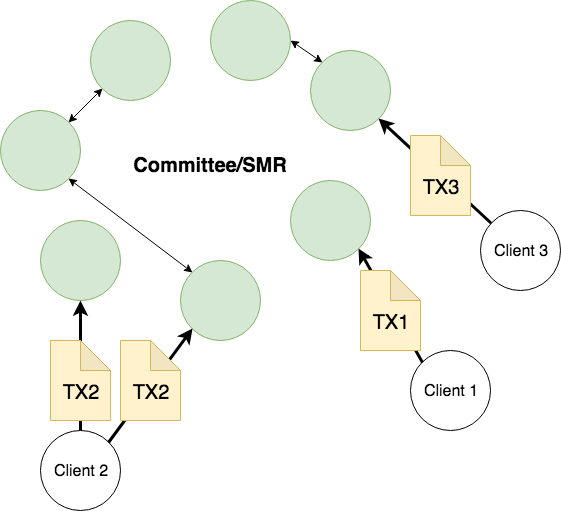
\includegraphics[scale=0.4]{Committee}
\caption{\textbf{Cхематическое изображение алгоритма}}
\label{fig:committee}
\end{figure}

\section{Рассматриваемая модель}
В данном разделе мы опишем модель, в которой работает предложенный алгоритм.

В рамках данной работы мы рассматриваем \textit{инклюзивную} (permissionless) модель, в которой:
\begin{itemize}
\item множество участников алгоритма не фиксировано
\item каждый участник может начать или закончить участие в алгоритме в любое время
\item каждый участник может быть однозначно идентифицирован его публичным ключом и каждый публичный ключ однозначно определяет участника
\item одно устройство может выступать как несколько участников
\end{itemize}

Участники могут быть либо \textit{честными} (honest), либо \textit{неисправными} (faulty).  Честный участник всегда следует предписанному алгоритму, неисправный же может предпринимать действия для нарушения корректной работы алгоритма.
В рамках данной работы мы будем считать, что в комитете находится не более $f$ неисправных участников, и размер комитета $n$ равен $3f+1$.

Что касается неисправных участников, мы считаем, что они могут пытаться скомпрометировать участников коммитета, пытаться подделывать их криптографические зашифрованные данные, взламывать устройство участника, и так далее. Однако, в рамках рассматриваемой модели, данные попытки занимают значительное время, что было формализовано в работе\cite{hybrid-consensus}, и носит название \textit{delayed adaptive adversary}.

Что касается модели сети, участиники сети соединены в пиринговую сеть (peer-to-peer), 
то есть кадждый участник поддерживает соединения с некоторыми другими участниками и обменивается с ними сообщениями. Будем считать, что любой участник может установить с любым другим участником соединение, по которому они могут обмениваться сообщениями. В следующих разделах мы разберем архитектуру сети более подробно.

В рамках данной модели сети будем считать, что отправленное сообщение может быть доставлено не более чем за время $\Delta$, которое является верхней границей на время доставки и известно заранее.
Обозначим $\delta$ как действительное время доставки сообщения от одного участника другому. 
Если время доставки превышает $\Delta$, считаем что участник неисправен, 
то есть $\delta \le \Delta$ для всех честных участников. 
Данная модель сети была формализована в статье Dwork \cite{Dwork:1988:CPP:42282.42283} и называется \textit{частично синхронная}(partially synchronous).

\section{Инклюзивный алгоритм SMR}
В данном разделе мы рассмотрим предложенный алгоритм, 
который является усовершенствованием алгоритма PBFT\cite{pbft} для решения задачи SMR в инклююзивной модели.
 
Так как состав комитета может меняться с течением времени, введем понятие \textit{конфигурация}, обозначающее состав комитета. Пронумеруем конфигурации, таким образом состав комитета ~--- это функция от его номера $c$, которую мы будем обозначать как $C(c)$. 
 
Один из участников в конфигурации является \textit{лидером}, который управляет алгоритмом SMR. 
Остальные участники конфигурации являются \textit{последователями}, которые проверяют и подтверждают действия лидера. Все честные последователи знают, какой участник является лидером.

Лидер в конфигурации может меняться с течением времени, при этом конфигурация может оставаться неизменной. Пронумеруем лидеров в пределах одной конфигурации, обозначив индекс лидера как $v$. Таким образом, лидер ~--- это функция от двух параметров $c$ и $v$: $L(c, v)$.

\subsection{Устойчивое состояние} \label{steady-state}
В данном разделе будет показано, как участники комитета приходят к консенсусу при неизменных $c$ и $v$. Данное состояние постоянности $c$ и $v$ называется \textit{устойчивым состоянием} (steady state).

Прежде всего, введем понятие \textit{лога примененных изменений} ~--- это индексируемый с нуля список, где нулевой элемент в списке ~--- первое примененное изменение, первый элемент ~--- следующее, и так далее. У каждого участника комитета имеется своя копия лога изменений, обозначим ее как $Log_C$, которые были применены к его локальной копии хранилища. \textit{Текущим слотом} будем называть $s$ равную длине $Log_C$. 
В ходе алгоритма, участники сообщения пытаются \textit{заполнить} текущий слот одинаковым сообщением, перейдя к следующему слоту.

Помимо лога и текущего слота каждый участник коммитета хранит следующие данные:
\begin{itemize}
\item номер текущей конфигурации $c$ и номер лидера $v$
\item список публичных ключей всех участников конфигурации с номером $c$ 
\item собственный секретный ключ
\item состояние, которое может обновляться инкрементально
\end{itemize}

Прежде чем перейти к описанию, введем следующее обозначение:
\[ \langle tag, a_1, a_2, ... a_n \rangle_X \] будем обозначать сообщение с тегом $tag$ и полями $a_1$, $a_2$..., $a_n$, подписанное секретным ключом участника $X$. Тег в данном случае ~--- это некоторая строка, которая отличает различные типы сообщений и делает невозможным переиспользование одного сообщения в качестве другого с точно такими же полями.

Теперь опишем как новое изменение попадает в лог участника комитета.

Пусть комитет находится в конфигурации с номером $c$ и лидером с номером $v$. 
Пусть лидер $L$ ($L = L(c, v)$) честный и хочет внести изменение $d$ в логи всех участников комитета. Алгоритм происходит в три раунда.

\textbf{Раунд 1. Предложение}. Лидер отправляет всем участникам конфигурации сообщение 
\[ \langle Propose, s, d \rangle_L \]

1.1 Каждый честный последователь $F$, получив сообщение, проверяет следующее:
\begin{itemize}
\item $s$ из сообщения равно локальным значению
\item подпись сообщения корректна и соответствует публичному ключу $L$
\item ранее ему не было прислано никакого другого $\hat d$ для $s$
\item валидно ли изменение $d$ и возможно ли применить его к состоянию
\end{itemize}

Если все вышеперечисленные проверки выполнились, $F$ присваивает $proposed_s := d$, в противном случае, $F$ игнорирует присланное сообщение. 
\vspace{10pt}

\textbf{Раунд 2. Подготовка}. Каждый честный последователь $F$, для которого выполнились все предыдущие проверки, отправляет лидеру $L$ сообщение 
\[ \langle Prepare, s, d \rangle_F \]

2.1 Лидер $L$, получив Prepare-сообщение, проверяет, что
\begin{itemize}
\item $s$ из сообщения равно локальным значению
\item подпись сообщения корректна и соответствует публичному ключу $F$
\item $d$ соответствует сообщению $Propose$ для $s$, отправленному им в предыдущем раунде
\end{itemize}
Если какая-то из проверок не выполнилась, лидер игнорирует присланное сообщение. 

2.2 Лидер дожидается $2f+1$ сообщений $Prepare$ (включая свое собственное) с одинаковыми значением $s$ и $d$ и формирует \textit{сертификат согласия} (Acceptance certificate), обозначим его как $\mathcal{P}$. Данный сертификат является гарантией того, что как минимум $2f+1$ участников (среди которых как минимум $f+1$ честных) пришли к согласию, что текущий слот $s$ должен быть заполнен изменением $d$.

Пока для простоты будем считать, что $\mathcal{P}$ ~--- это кортеж
$$(s, d, \sigma_1, \sigma_2, ..., \sigma_{2f+1})$$
где $Prepare$ ~--- это тег, а $\sigma_i$ ~--- подпись $Prepare$ сообщения $i$-го приславшего участника (включая самого лидера). 
В последующих разделах, формирование сертификата $\mathcal{P}$ будет проанализировано и улучшено.

2.3 После этого лидер отправляет всем последователям  $\mathcal{P}$

2.4 Каждый честный последователь $F$, получив сертификат, проверяет следующее:
\begin{itemize}
\item $s$ из сообщения равно локальному значению
\item $proposed_s = d$
\item все подписи в $\mathcal{P}$ корректны
\end{itemize}
\vspace{10pt}

Если все проверки выполнинились, то участник запоминает данный сертификат в $acceptance_s := \mathcal{P}$.
\vspace{10pt}

\textbf{Раунд 3. Применение}.
Каждый честный последователь $F$, для которого выполнились все предыдущие проверки, отправляет лидеру $L$ сообщение 
\[ \langle Commit, s, d \rangle_F \]

3.1 Лидер $L$, получив $Commit$-сообщение, проверяет его аналогично шагу 2.1.
Если какая-то из проверок не выполнилась ~--- лидер игнорирует присланное сообщение. 

3.2 Лидер дожидается $2f+1$ сообщений $Commit$ (включая свое собственное) с одинаковыми значением $s$ и $d$ и формирует \textit{сертификат применения} (Commit certificate), обозначим его как $\mathcal{C}$.
$$\mathcal{C}=(s, d, \sigma_1, \sigma_2, ..., \sigma_{2f+1})$$

3.3 После этого лидер отправляет всем последователям  $\mathcal{C}$

3.4 Каждый честный последователь $F$, получив сертификат, проверяет его аналогично шагу 2.4.
Если все проверки выполнились ~--- последователь добавляет изменение $d$ в свой лог и  применяет изменение $d$ к своему локальному состоянию.
\vspace{10pt}

Следует отметить, что лидер следует всем шагам алгоритма действуя и как лидер, и как последователь. За исключением того, что он не отправляет сообщения самому себе.

Будем называть сертификат \textit{корректным}, если все подписи в нем корректны.
Стоит обратить внимание, что вообще говоря два последователя $F_1$ и $F_2$ могут получить разные корректные сертификаты согласия $\mathcal{P}_1$ и $\mathcal{P}_2$ и/или применения $\mathcal{C}_1$ и $\mathcal{C}_2$, однако, это не нарушает корректность алгоритма, при условии что сертификаты корректны.
То есть лидер может дождаться более чем $2f+1$ $Prepare$/$Commit$ сообщения и сформировать каждому последователю корректный сертификат, отличный от других.

Также, если лидер отправляет последователю сертификат для $s$, в то время как последователь уже имеет корректный сертификат для $s$, то последователь игнорирует присланный.

\subsection{Реконфигурация}
В данном разделе будет описано, как комитет переходит в новую конфигурацию, то есть как обновляется состав комитета. Данный шаг называется реконфигурация ~--- то есть изменение конфигурации.

Cхема реконфигурации состоит в том, что \textit{майнеры} ~--- участники сети, которые хотят вступить в комитет, совершают работу по решению некоторого \textit{паззла}. После того как решение найдено, майнер публикует данное решение в комитет, каждый участник комитета проверяет найденное решение, и отвечает майнеру сообщением подтверждением, что решение корректно и участник готов принять его в комитет.
После чего, текущий лидер комитета предлагает изменение, которое добавляет майнера в комитет.

Формально, решение паззла ~--- это некоторое число $\phi$, что:
$$\mathcal{H}(puzzle_c, pk, \phi) \le target$$
где $\mathcal{H}$ ~--- криптографически стойкая хэш-функция, $puzzle_c$ ~--- это некоторая величина, зависящая от $c$, называемая \textit{паззлом}, $pk$ ~--- публичный ключ майнера, $target$ ~--- некоторое число, которое задает сложность вычисления.

Другими словами, майнеры выполняют доказательство выполненной работы (PoW), подобно тому, как это делается в Bitcoin.  Число $target$ выбирается так, чтобы поиск числа $\phi$ примерно занимал некоторое время $D$, намного большее $\Delta$. Скажем, $D$ равное 10 минутам, как и в Bitcoin подойдет.  $target$ также меняется со временем, и зависит от частоты нахождения предыдущих значений $PoW$, более подробно с тем, как выбирается $target$ можно познакомиться в оригинальной статье [ссылка].
Как формируется число $puzzle_c$ будет рассказано далее в этом разделе, на данный момент важно лишь то, что паззл зависит от номера конфигурации. Сосредоточимся более подробно на том, как майнер добавляется в комитет.

Майнера, который нашел число $\phi$, будем называть \textit{кандидатом}.
Прежде всего, каждый участник комитета для конфигурации $c$ хранит множество известных ему кандидатов $Q_c$.
\vspace{10pt}

Итак, после того, как майнер $W$ нашел число $\phi$, он отправляет всем участникам комитета сообщение
 \[ \langle Candidate, c, puzzle_c, pk, \phi \rangle_W \]
 
Участник $M$, получивший данное сообщение, выполняет следующую последовательность шагов:

1. Берет эксклюзивную блокировку $B$ на чтение данных. То есть откладывает обработку сообщения от лидера $L(c, v)$ до тех пор, пока блокировка не будет отпущена. 

2. Проверяет, что выполняется все из следующего:
\begin{itemize}
\item корректность подписи $W$ 
\item корректность решения пазла, то есть что $\mathcal{H}(puzzle_c, pk, \phi) \le target$
\item $c$ из сообщения равно локальному значению
\end{itemize}

3. Засекает таймер $T$ на $5\Delta$ и отправляют кандидату $W$ сообщение:
 \[ \langle Status, c, v, s, pk \rangle_M \]
где $c$, $v$~--- локальные  $c$, $v$, $pk$~--- публичный ключ $W$.
\vspace{10pt}

После того как $W$ получает $2f+1$ корректно подписанных $Status$ сообщений с одинаковыми $(c, v)$, он вычисляет $s^{*}=max(s_1, s_2,..., s_{2f+1})+2$, где $s_i$~--- слоты из $Status$ сообщений.
Далее отправляет всем участникам запрос на подтверждение слота:
 \[ \langle ReserveSlot, c, v, s^{*} \rangle_W \]
 
\noindent Участник $M$, получивший это сообщение, проверяет:
\begin{itemize}
\item корректность подписи W
\item $c$ и $v$ равны локальным значениям
\item $proposed_{s^{*}}$ еще не заполнено никаким изменением $d'$
\end{itemize} 
После чего отправляет в ответ $W$:
 \[ \langle ConfirmSlot, c, v, s^{*}, pk \rangle_M \]
где $pk$~--- публичный ключ $W$.
\vspace{10pt}

После получения $2f+1$ корректно подписанных $Confirm$, с одинаковыми значениями $c$, $v$ и $s^{*}$,
формирует и отправляет всем участникам комитета \textit{сертификат кандидата} $\mathcal{S}$:

$$\mathcal{S}=(c, v, s^{*}, pk, \sigma_1, \sigma_2,..., \sigma_{2f+1})$$
$\sigma_i$ ~--- подписи $ConfirmSlot$ сообщений.
\vspace{10pt}

Участник $M$, получивший данное сообщение, выполняет шаги : 

1. Проверяет подписи $ConfirmSlot$ сообщений $\sigma_i$.

2. Добавляет $\mathcal{S}$ в $Q_c$.

3. Отправляет данный сертификат всем остальным участникам комитета.

4. Снимает блокировку на ресурсы $B$.

Если кандидат не успевает прислать сертификат $\mathcal{S}$ до истечения таймера $T$, блокировка $B$ снимается.

Данная процедура во-первых гарантирует, что либо все честные участники, либо ни одного (в зависимости от честности действий кандидата) узнают о новом кандидате, а во-вторых что как минимум $f+1$ честных участников придут к консенсусу о $s^{*}$.

После того, как все честные участники, в том числе и лидер $L(c, v)$, узнали о кандидатах, претендующих на добавление в комитет, участники ожидают от лидера, что в скором времени лидер предложит изменение, которое изменит конфигурацию комитета. А именно, каждый раз, когда участник получает $Propose$ сообщение, помимо проверок описанных в  разделе \ref{leader-change}, он проверяет, что данное сообщение $Propose$ содержит тех, и только тех кандидатов из $Q_c$, для которых выполяется $s^{*} = s$, где $s$~--- слот из $Propose$ сообщения. Если же это условие не выполняется, участник игнорирует данное $Propose$ сообщение.

Изменение реконфигурации $d_{rec}$ формально описывается следующим образом:
$$d_{rec}=(c, puzzle_c, (pk_1, \phi_1, \sigma_1), (pk_2, \phi_2, \sigma_2),...,(pk_k, \phi_k, \sigma_k))$$
где $k$~--- количество кандидатов, $\sigma_i$~--- подпись $Candidate$ сообщения.

Как только $d_{rec}$ будет применено и попадет в лог применений, необходимо произвести реконфигурацию.
Реконфигурация задается функцией $\Phi$ из изменения реконфигурации в список кандидатов. Данная функция определяет каких кандидатов и в каком порядке необходимо добавить в комитет, следовательно, столько же самых давних участников должны покинуть его. Для простоты рассмотрим $\Phi$, которая возвращает кандидата, у которого решение пазла является наименьшим, то есть $\mathcal{H}(puzzle_c, pk, \phi)$ наименьше, а при равенстве, выберем c наименьшим $pk$.

Итак, после того как участник $M$ получил сертификат применения $d_{rec}$, он выполняет следующие шаги:

1. Отправляет его всем остальным участникам

2. Проверяет, является ли он самым давним участником, покидает комитет и перестает выполнять дальнейшие шаги. 

В противном случае выполняет последующие шаги алгоритма:

3. Вызывает процедуру актуализации лога применений (которая будет описана в разделе \ref{act_log})

4. Добавляет $d_{rec}$ в лог применений

5. Вычисляет $pk=\Phi(d_{rec})$

6. Добавляет кандидата $pk$ в список участников комитета и убирает самого старого из списка

7. Заводит $Q_{c+1} := \{\}$

8. Отправляет вновь добавленному кандидату сообщение $\langle Welcome, c+1, \mathcal{C} \rangle_M$, где $\mathcal{C}$~--- сертификат применения $d_{rec}$.

9. Присваивает $L(c+1, 0):=pk$.

10. Вычисляет $puzzle_{c+1}=$ \textbf{TODO}.

11. Увеличивает $c$ на один и обнуляет $v$

12. Запускает процедуру актуализации лога применений для сертификата $d_{rec}$, которая описана в разделе \ref{act_log}.

После того, как кандидат $W$ получит $f+1$ корректное $Welcome$ сообщение, он начинает действовать как лидер комитета. В данный момент реконфигурация считается проведенной успешно и комитет переходит в новое устойчивое состояние.

\subsection{Смена лидера} \label{leader-change}
В данном разделе будет описано, как участники комитета переходят к лидеру с номером $v+1$, если текущий лидер препятствует прогрессу системы. Прежде всего опишем, как последователь обнаруживает \textit{отстутствие прогресса}.

Будем считать, что лидер производит изменения довольно часто. В следующих разделах будет пояснено, почему данное предположение корректно.

После очередного применения некоторого изменения $d$ или смены лидера последователь $M$ запускает таймер на время $6\Delta$ ~--- за это время честный лидер должен успеть провести 3 раунда описанных выше, и последователь должен получить следующее изменение.
Данная величина получена из следующих соображений, что последователи обмениваются с лидером пятью сообщениями, и так как мы считаем, что в рамках данной модели сообщение отправленное честным участником не должно идти дольше времени $\Delta$, данная процедура не должна занять больше $5\Delta$. Делая поправку на погрешность, а также учитывая то, что проверка сообщений также занимает некоторое время, добавляем к этом времени еще $\Delta$.

После того, как последователь $M$ обнаружил отсутствие прогресса, то есть состояние, при котором текущий лидер не предложил новое измнение за время $6\Delta$, последователь переходит в \textit{состояние смены лидера}.
Результат выхода из этого состояния будет следующее устойчивое состояние с новыми $c$ и $v$.
Цель описанного далее процесса~--- сформировать сертификат \textit{устойчивого состояния}:
$$\mathcal{W}=((c, v', s, \hat{\mathcal{P}}_1,\hat{\mathcal{P}}_2,...,\hat{\mathcal{P}}_{2f+1}, Q_1, Q_2,..., Q_{2f+1}, \sigma_1, \sigma_2,..., \sigma_{2f+1}), \varkappa_1, \varkappa_2,..., \varkappa_{2f+1})$$ 

Данный сертификат содержит значения $c, v', s$, на которых участники согласовываются, переходя в новое устойчивое состояние, а также о последних имеющихся у участников сертификатах согласия и множествах кандидатов.

Итак, после того, как участник $M$ перешел в состояние смены лидера, он проделывает следующее:

1. Перестает принимать сообщения с тегом отличным от $LeaderChange$ и $NewLeader$

2. Отправляет сообщение новому лидеру $L(c, v+1)$:
\[ \langle LeaderChange, c, v+1,  \hat{\mathcal{Y}} \rangle_M \]
где $\hat{\mathcal{Y}}$~--- один из сертфикатов $\hat{\mathcal{C}}$ или $\hat{\mathcal{W}}$, имеющий наибольшее значения слоа, при равенстве $\hat{\mathcal{W}}$, $\hat{\mathcal{C}}$~--- это последнний сертификат применения, $\hat{\mathcal{W}}$~--- \textit{устойчивого состояния} (будет описан далее), полученные $M$.

3. Засекает таймер на $7\Delta$.

4. Если таймер истек, $M$ не перешел в новое устойчивое состояние, то он повторяет шаги 2 и 3 для следующего лидера $v+2$. Данный шаг будет повторяться до тех пор, пока $M$ не окажется в устойчивом состоянии.
\vspace{10pt}

После того, как новый лидер $L(c, v')$ получит $2f+1$ корректно подписанных сообщений $LeaderChange$ с одинаковыми $c$ и $v'$  (включая свое), проверяет корректность сертификата $\hat{\mathcal{Y}}$  и формирует и отправляет сертификат \textit{актуализации} $\mathcal{A}$
$$\mathcal{A}=(c, v', \hat{\mathcal{Y}}_1,  \hat{\mathcal{Y}}_2,...,  \hat{\mathcal{Y}}_{2f+1}, \sigma_1, \sigma_2,..., \sigma_{2f+1})$$
где $\sigma_i$ ~--- это подпись $LeaderChange$ сообщения $i$-го приславшего участника.
\vspace{10pt}

Получив этот сертификат, участник $M$:

1. Проверят его корректность

2. Выбирает $\hat{\mathcal{Y}}^{*}$ из $\mathcal{A}$ с наибольшим занчением слота $s^{*}$.

3. Запускает процедуру актуализации лога применений (описанную в следующем разделе) с текущим слотом и $\hat{\mathcal{Y}}^{*}$. 

4. Если $\hat{\mathcal{Y}}^{*}$ это сертификат устойчивого состояния, то последователь обновляет свой $acceptance_{s_P^{*}} :=  \hat{\mathcal{P}}^{*}$, где $\hat{\mathcal{P}}^{*}$~--- это $\hat{\mathcal{P}}_i$ с наибольшим значением слота в нем.

5. После чего последователь отправляет $L(c, v')$ сообщение:
\[ \langle Sync, c, v',  s, \hat{\mathcal{P}},  Q_c \rangle_M \]
\vspace{10pt}

Получив $2f+1$ $Sync$ сообщений с одинаковыми $c, v',  s$, новый лидер $L(c, v')$ формирует и отправляет подготовительный сертификат устойчивого состояния:
$$\mathcal{V}=(c, v', s^{*}, \hat{\mathcal{P}}_1,\hat{\mathcal{P}}_2,...,\hat{\mathcal{P}}_{2f+1}, Q_1, Q_2,..., Q_{2f+1}, \sigma_1, \sigma_2,..., \sigma_{2f+1})$$
$\sigma_i$ ~--- это подпись $Sync$ сообщения $i$-го приславшего участника.

Участник, получив его, проверяет, что его слот совпадает с $s$ из сертификата, а также корректность всех $\hat{\mathcal{P}}_i$, после чего отправляет свою подпись $\varkappa$, тем самым подтверждая, что он осведомлен о данном подготовительном сертификате. Лидер $L(c, v')$ собрав $2f+1$ подписей наконец формирует сертификат устойчивого состояния участникам:
$$\mathcal{W}=(\mathcal{V}, \varkappa_1, \varkappa_2,..., \varkappa_{2f+1})$$
\vspace{10pt}

После того как последователь $F$ получил $\mathcal{W}$, он проверяет следующее:
\begin{itemize}
\item подпись $NewLeader$
\item значение $c$ из сертификата совпадает с локальным
\item $v'$ строго больше локального $v$
\item корректность всех $\hat{\mathcal{P}}_i$
\item корректность всех подписей $\sigma_i$ для $Sync$ сообщений
\item корректность всех подписей $\varkappa_i$ $\mathcal{V}$
\end{itemize}

Если хотя бы одна из проверок не выполнилась, $F$ игнорирует сообщение. В противном случае:

1. Находит $s_P^{*}$ как наибольшее значение слота из $\hat{\mathcal{P}}_i$, а также соответствующий сертификат $\hat{\mathcal{P}}^{*}$.

2. Проводит процедуру актуализации лога применений

3. $F$ обновляет свое $Q_c := \bigcup\limits_{i=1}^{2f+1} Q_i$.

4. Значение $v$ значением $v'$ и тем самым \textit{принимает} нового лидера.

5. Обновляет $acceptance_{s_P^{*}} := \hat{\mathcal{P}}^{*}$ и  $steadyState_{s^{*}} := \mathcal{W}$

6. В случае если $s^{*}+1=s_P^{*}$, отправляет
\[ \langle Commit, s_P^{*}, d^{*} \rangle_F \]
и дожидается сертификата применения от $L(c, v')$, после чего участник переходит в новое устойчивое состояние, иначе по истечению таймера переходит к смене лидера.

7. Если условие в шаге 6 не выполнилось, то есть $s^{*}=s_P^{*}$, то участник переходит в новое устойчивое состояние после шага 6.

Стоит обратить внимание, что участник $F$ может уже иметь сертификат применения для $s_P^{*}$, $d^{*}$, однако в случае выполнения  шага 6, он все равно отправляет $Commit$ сообщение.

Процедура смены лидера несет две цели: достигнуть консенсуса о новом лидере, а также актуализировать логи всех честных участников, устраняя отставание, которое мог создать предыдущий лидер.

В следующей главе будет доказано, что либо $s^{*}=s_P^{*}$, либо $s^{*}+1=s_P^{*}$, то есть либо сертификат согласия соответствует сертификату применения, либо сертификат согласия соответствует предложенному предыдущим лидером изменению.

\subsection{Процедура актуализации лога применений} \label{act_log}
Процедура актуализации лога применений необходима для устранения отставания участника комитета.
Она принимает на вход текущий слот участника $s$ и сертификат согласия или применения $\mathcal{D}$, имеющийся у участника.

Обозначим $s$ текущий слот участника комитета $M$, а $s_k$ номер слота из сертификата. Если $s \le s_k-1$, тогда $M$ отправляет любым $f+1$ участникам из сертификата 
\[ \langle RequestCommits, s, s_k-1 \rangle_M \]
тем самым запрашивая изменения соответствующие слотам $s, s+1,..., s_k-1$

Участник $M'$, получивший данное сообщение и имеющий сертификаты применения для соответствующих слотов, отправляет их в ответ
\[ \langle ReponseCommits, \mathcal{C}_s, \mathcal{C}_{s+1},...,\mathcal{C}_{s_k-1} \rangle_{M'} \]

Получив их $M$ проверяет корректность каждого из них и применяет изменения к состоянию, добавляя их после этого в лог применений. Таким образом процедура гарантирует, что в лог применений будет заполнен по слот $s_k-1$ включительно.

\subsection{Стартовый запуск}

\section{Взаимодействие комитета с клиентами}

\section{Микроблоки}

\section{Уменьшение размера сертификата}



%-*-coding: utf-8-*-

\chapter{Анализ предложенного алгоритма}  \label{chapter3}

\section{Модель и определения}
Прежде всего опишем модель, в которой будут проводиться следующие рассуждения, доказательства лемм и теорем.

Определим \textit{события} в системе. Событиями будем считать:
\begin{itemize}
\item отправку сообщения
\item получение сообщения
\item запуск таймера
\item остановку таймера
\end{itemize}

Будем считать, что событие отправки сообщения происходит до его получения, запуска таймера до его остановки, а также, что события одного участника могут быть линейно упорядоченны.

В итоге мы получили систему на основе событий с полным порядком. В данной системе можно ввести понятие \textit{согласованного среза}[ссылка]. Также введем в данной системе глобальное время. Каждому событию в системе можно сопоставить некоторый глобальный момент времени, причем будем считать, что двум событиям одного участника соответствуют разные моменты времени. Заметим, что все события, которые произошли до некоторого момента времени $t$, образуют согласованный срез. Таким образом, если некоторое утверждение верно для любого среза, то оно также верно и для и для всех событий до момента времени $t$.

Прежде всего, каждый участник имеет состояние, в которое входят следующие переменные:
\begin{itemize}
\item leaderChange :: Bool
\end{itemize}

Обозначим состояние $i$-го участника в момент времени $t$ как $S_i(t)$, а состояние всей системы $S(t)$. 
$S(t)=\{S_1(t), S_2(t),..., S_{3f+1}(t)\}$. Также введем обозначение $variable^i(t)$ значение переменной $variable$ у участника $i$ в момент времени $t$.
Обозначим состояние $i$-го участника в согласованном срезе $C$ как $S_i(C)$, аналогично $S(C)$ и $variable^i$.
Если $S^i$, $S$ и $variable^i(t)$ используется без указания времени или среза, то предполагается, что $t$ или $C$ ясны из контекста, либо для любых $t$ и $C$.

Будем считать, что честные участники изменяют их состояния согласно описанному алгоритму, в то время как нечестные могут изменять произвольно.

Злые участники \textbf{TODO}.

\textit{Определение.} Будем называть изменение $d$ \textit{оседлым} в слоте $s$, если у как минимум $f+1$ честного участника $acceptance_s$~--- это корректный сертификат согласия для $(c, v, s, d)$.

\textit{Определение.} Будем считать, что честный участник $i$ находится в \textit{состоянии смены лидера}, если $leaderChange^i = True$.

\textit{Определение.} Будем считать, что честный участник $i$ находится в \textit{устойчивом состоянии}, если $leaderChange^i = False$.

\textit{Определение.} Состояние системы $S$ называется \textit{устойчивым состоянием}, если не более $f$ честных участников находятся в состоянии смены лидера. 
%и как минимум $f+1$ честных участников, находящихся в устойчивом состоянии, имеют одинаковое значение $(c^i, v^i)=(c,v)$.

Будем говорить \textit{устойчивое состояние $(c, v)$}, имея ввиду $(c, v)$ из определения.

Если система или участник не находится в устойчивом состоянии, будем говорить, что они находится в \textit{неустойчивом} состоянии.

\section{Базовые свойства}
В данном разделе будут доказаны некоторые базовые свойства, который будут использоваться в дальнейшем.

\textbf{\textit{Свойство 1.}} \textit{Весь жизненный цикл системы разбивается на последовательность времен
$T_0 < T_1 < T_2 < T_3 < ...$, $T_0=0$, где в полуитервалах $[T_{2k}...T_{2k+1})$ система находится в устойчивом состоянии, а в полуинтервалах $[T_{2k+1}...T_{2k+2})$ в неустойчивом.}
Это очевидно следует из того, что количество участников, который находятся в состоянии смены лидера либо не больше $f$, либо больше $f$. $\square$.
\vspace{10pt}

\textbf{\textit{Свойство 2.}} \textit{Значение $(c^i, v^i)$ не убывает со временем.}
Это очевидно следует из того, что на протяжении алгоритма, значения $с$ и $v$ только увеличиваются. $\square$.
\vspace{10pt}

\textbf{\textit{Свойство 3.}} \textit{В любой момент времени не может существовать более одного сертификата согласия с одинаковой тройкой значений $(c, v, s)$, но для разных изменений.} 

Предположим, что существуют два сертификата согласия $\mathcal{P}_1$ и $\mathcal{P}_2$ с одинаковыми $(c, v, s)$, но разыми $d_1$ и $d_2$. 
Обозначим за $A$ множество участников отправивших $Prepare$ сообщения для  $\mathcal{P}_1$ ($|A|=2f+1$), за $B$ ($|B|=2f+1$) сообщения для $\mathcal{P}_2$. $|A \cap B| \ge f+1$, отсюда следует, что в пересечении найдется как минимум один честный участник,  обозначим его за $x$. Получаем, что $x$ отправил два $Prepare$ сообщения с разными $d_1$ и $d_2$, но одинаковыми $(c, v, s)$. Однако, это противоречит проверке 1.1 из раздела \ref{steady-state}. $\square$
\vspace{10pt}

\textbf{\textit{Свойство 4.}} \textit{В каждом устойчивом состоянии существует такой согласованный срез $C$, для которого выполняется, что у всех честных участников, кроме может быть $f$ из них, $s^i$ равны некоторому значению $s$ и $acceptance^i_s$ одинаковы.}

Это очевидно верно для устойчивого состояния $[T_0...T_1)$, срез $C$ можно взять по $T_0$.

Рассмотрим некоторое устойчивое состояние, а также предыдущее ему состояние смены лидера.
Если хотя бы у одного честного участника $i$ значение $leaderChange$ стало $True$, это значит, что он получил сам и отправил другим $\mathcal{W}$. Получая $\mathcal{W}$, участник актуализирует лог вплоть до $s^{*}$ и присваивает $acceptance_{s_P^{*}} := \hat{\mathcal{P}}^{*}$. Если в какой-то момент времени, состояние стало устойчивым, значит у не более чем $f$ честных участников $leaderChange = False$, следовательно, для остальных существовал такой момент времени $t_i$, в который $s^i$ был равен $s^{*}$ и $acceptance_{s_P^{*}}$ равен $\hat{\mathcal{P}}^{*}$. Возьмем эти моменты времени $t_i$ в качестве среза $C$. $\square$

\section{Консистентность алгоритма}
В данном разделе будет дано определение \textit{консистентности} (Consistency)\cite{hybrid-consensus} и доказано, что предложенный алгоритм обладает этим свойством.

Будем считать, что алгоритм обладает свойством \textit{общего префикса}, если в любой момент для любых двух честных участников комитета (возможно одного и того же) $i$ и $j$ выполняется: либо $Log_{C_i}$ префикс $Log_{C_j}$, либо $Log_{C_j}$ префикс $Log_{C_i}$. Считаем, что $x$ префиксом самого себя и $\emptyset$ префиксом $x$.

Будем считать, что честный участник удовлетворяет свойству \textit{самоконсистентности}, если выполняется: пусть участник честный во время $t$ и $t' \ge t$, $Log_{C_i}$~--- лог в момент времени $t$, $Log'_{C_i}$~--- в момент времени $t'$, тогда верно, что $Log_{C_i}$ префикс $Log'_{C_i}$.

Будем называть алгоритм \textit{консистентным}, если для него выполняется свойство общего префикса и для любого участника выполняется свойство самоконсистентности.
 
Далее будет приведено доказательство консистентности предложенного алгоритма.

\textbf{\textit{Лемма 1.}} \textit{В любой момент времени для любого слота $s$ существует не более одного оседлого изменения $d$.}

Предположим, что существуют два оседлых изменения $d_1$ и $d_2$ в слоте $s$. Рассмотрим сертификат согласия $\mathcal{P}_1$ любого участника для $d_1$ и сертификат согласия $\mathcal{P}_2$ любого участника для $d_2$. Обозначим за $(c_1, v_1)$ значения $c$ и $v$ из первого сертификата, и $(c_2, v_2)$ из второго.

Обозначим за $A$ множество участников отправивших$Prepare$ сообщения для  $\mathcal{P}_1$ ($|A|=2f+1$), за $B$ ($|B|=2f+1$) сообщения для $\mathcal{P}_2$. $|A \cap B| \ge f+1$, отсюда следует, что в пересечении найдется как минимум один честный участник,  обозначим его за $x$. Получаем, что $x$ отправил два $Prepare$ сообщения с разными $d_1$ и $d_2$: одно с $(c_1, v_1, s)$ и второе с $(c_2, v_2, s)$.

Допустим, что $c_1 = c_2$ и  $v_1 = v_2$. Тогда получаем противоречие со Свойством 3.

Допустим теперь, что $c_1 < c_2$. Это бы значило, что $x$ между отправками $Prepare$ сообщений должен был перейти в другую конфигурацию. Сделать он это может только добавив в свой лог $\mathcal{C}$ с $d_{rec}$, тем самым увеличив свое значение слота, но тогда бы он не смог отправить второе $Prepare$ сообщение для того же самого $s$, что и первое. Аналогично для случая $c_2 < c_1$.

Допустим теперь, что $c_1=c_2=c$ и $v_1 < v_2$. Пусть $\mathcal{P}_1$ стал оседлым первым в момент времени  $T$. Пусть на данный момент в последнем участнике, принявшим $\mathcal{P}_1$ значение конфигурации и номера лидера были $(c, v^i) < (c, v_2)$, тогда в следующем устойчивом состоянии $d_1$ должно быть применено в лог изменений как минимум у $f+1$ участников, и соотвественно, их значение слота будет больше $s$, что не позволит им отправить $Prepare$ сообщение для $s$. $\square$
\vspace{10pt}

\textbf{\textit{Лемма 2.}} \textit{Если изменение $d$ стало оседлым в $s$ в устойчивое состояние то $(c, v)$ сертификата согласия строго больше $(c^j, v^j)$ сертификата согласия для неоседлого в слоте $s$ изменения $d'$ ($d \ne d'$).}

Если изменение стало оседлым в устойчивом состоянии, то это значит, что как минимум у $f+1$ честного участника $(c^i, v^i)$ равно значению в сертификате $(c, v)$. И так как $(c^i, v^i)$ увеличивается со временем по Свойству 2, все предыдущие сертификаты согласия имеют $(c^j, v^j)$ меньше либо равное $(c^i, v^i)$, но $(c^j, v^j)$ не может быть равно $(c^i, v^i)$ так как это бы противоречило Свойству 3.
$\square$
\vspace{10pt}

\textbf{\textit{Лемма 3.}} \textit{Если в некоторый момент времени $T$ для слота $s$ существует некоторое оседлое изменение $d$, то данное изменение в конечном счете окажется в логе применения всех честных участников в слоте $s$.}

Пускай не теряя общности, $t \le T$~--- это первый момент времени, в который $d$ стало оседлым в $s$.

Пусть в момент времени $t$ система находится в устойчивом состоянии. Чтобы оставаться в нем, лидер  должен за некоторое ограниченное время отправить как минимум $f+1$ честным участникам $\mathcal{C}$ для $s, d$, иначе же система перейдет в состояние смены лидера. Отметим, что у лидера нет другой опции, кроме как уведомить минимум $f+1$ честных участников о $\mathcal{С}$ для $s, d$, потому что $f+1$ честный участник ожидает только его, так как они получили $\mathcal{P}$ и отправили свое $Commit$ сообщение.

Если существуют как минимум $f+1$ честных участников, которые имеют $\mathcal{C}^i$ для слота не меньшего чем $s$, тогда очередная процедура реконфигурации распространит среди всех честных участников некоторый $\mathcal{C}'$ со слотом большим $s$. Таким образом, честные участники, для которых неизвестен $\mathcal{С}$ для $s, d$, смогут получить его в процедуре актуализации логов на шаге 3.3 реконфигурации.

Теперь рассмотрим случай, когда в момент времени $T$ система находится в состоянии смены лидера ($T_{2k+1} \le T < T_{2k+2}$). Не теряя общности, возьмем наименьшее такое $T$, для которого все еще выполняется $T_{2k+1} \le T < T_{2k+2}$.

Если $T= T_{2k+1}$, то есть изменение $d$ было оседлым в $s$ с $\mathcal{P}$ для $(c, v)$ до начала состояния смены лидера, тогда в сертификате $\mathcal{W}$, полученном для следующего устойчивого состояния, $\mathcal{P}^{*}$ неизбежно будет для $c, v, s, d$, так как для формирования $Election$ сообщения необходимо как миниум $2f+1$ $LeaderChange$ сообщение, следовательно, обязательно присутствие как минимум одного $\mathcal{P}$ для $c, v, s, d$. Также принимаем во внимание, что по Лемме 1 не может существовать другого оседлого значения, и по Лемме 2 любой другой сертификат имеет $(c^j, v^j)$ меньшее, чем $(c, v)$. С другой стороны, система не перейдет в новое устойчивое состояние до тех пор, пока как минимум $f+1$ честный участник не получит $\mathcal{C}$ для $s, d$. Учитывая то, что среди $f+1$ лидеров, которым отправят $LeaderChange$, будет как минимум один честный, рано или поздно это произойдет. А далее по уже описанному случаю.

Если же  $T > T_{2k+1}$, это означает, что $d$ могло стать оседлым только на шаге 3.5 процедуры смены лидера. Тогда в следующем устойчивом состоянии как минимум $f+1$ честный участник будет иметь сертификат $acceptance_s = \mathcal{P}^{*}$, и следовательно, как минимум $f+1$ честный будут иметь $\mathcal{C}$ для $s, d$. А далее доказательство для уже описанного выше случая.
$\square$
\vspace{10pt}

\textit{Следствие из Леммы 3.} Если хотя бы один честный участник имеет сертификат применения $\mathcal{C}$ для изменения $d$, то  изменение $d$ неизбежно окажется в логе применения всех честных участников в слоте $s$. 

Это следует из того, что как минимум $f+1$ честных участнкиков, отправивших $Commit$ сообщение для $\mathcal{C}$, имеют сертификат согласия для $d$ и $s$. $\square$
\vspace{10pt}

\textbf{Теорема.} \textit{В любой момент времени логи честных участников консистентны.}

Предположим, что в некоторый момент времени существуют различные участники $i$ и $j$, такие что, существует $s$, для которого выполняется, что изменение из $Log_{C_i}[s]$ неравно изменению из $Log_{C_j}[s]$. Тогда существовал некоторый момент времени, в который либо изменение $Log_{C_i}[s]$, либо изменение $Log_{C_j}[s]$ оказалось у честного участника, отсюда по следствии из Лемме 3 получаем, что в конечном итоге это изменение должно было оказаться в слоте $s$ у всех честных участников.

Свойство самоконсистентности очевидно, так как в описанном алгоритме изменения не удаляются из лога применений и не модифицируются, а только добавляются в него. $\square$

\section{Прогресс алгоритма}
\noindent Следующее свойство ~--- это свойство \textit{прогресса} (Liveness) \cite{hybrid-consensus}:
пусть честный участник получил транзакцию во время $t$, тогда данная транзакция будет добавлена в хранилище всеми \textit{честными} участниками не позднее $t + T_{confirm}$.

Данное свойство использует параметр $T_{confirm}$, предполагается что данный параметр постоянен на протяжении всего времени и известен зараннее.

\section{Отзывчивость алгоритма}

\startconclusionpage

В рамках данной работы был предложен алгоритм консенсуса для распределенных геореплицируемых систем.
Два основных преимущества предложенного решения по сравнению с существующими состоят в том, что в алгоритме не может быть вилок, таким образом он обладает строгой консистентностью, второе, но не менее важное преимущество~--- уменьшены затраты на коммуникацию между участниками системы.

Алгоритм был рассмотрен в контексте разработки криптовалют, подробно описан в главе 2, а также проанализирован в главе 3. В результате анализа было доказано, что алгоритм обладает консистентностью и  обеспечивает прогресс системы, также были приведены оценки на ожидаемое время обработки транзакций. Тем самым были продемонстрировано, что алгоритм предоставляет необходимые гарантии и показана жизнеспособность.

Основным недостатком предложенного решения является то, что в его основе лежит подход на основе доказательства проделанной работы, который требует использования большого количество энергии. Другим же  недостатком является требование на нахождение в сети как минимум $2f+1$ активных участников. Данные проблемы могут быть решены используя другие подходы, такие как доказательство доли владения и другие, которые лишены данных проблем, хотя и обладают другими.

В заключении, хочется отметить, что предложенный в данной работе подход~--- это еще один шаг в сторону более устойчивых и быстрых алгоритмов консенсуса. Алгоритм не лишен недостатков, но многие из них обозначены в рамках работы и могут быть устранены во время дальнейшей  его разработки.

\printmainbibliography

%\appendix

%\input{appendicies/adagrad_1.tex}
%\input{appendicies/adagrad_2.tex}
%\input{appendicies/adam_1.tex}
%\input{appendicies/adam_2.tex}
\end{document}
